\chapter{Análise}
\label{chap:Analise}

Este capítulo define as funcionalidades que debe proporcionar SintromApp e as condicións baixo as que debe operar. Para describir o comportamento da aplicación escolleuse un enfoque baseado en \textbf{casos de uso}, xa que permite identificar con claridade os actores que interactúan co sistema e os principais obxectivos que poden realizar mediante a aplicación.

A descrición complétase coa definición dos requisitos funcionais e non funcionais. Estes elementos servirán posteriormente como referencia para o deseño da arquitectura e para a definición das probas da aplicación.

\section{Alcance do sistema}
\label{sec:alcance-sistema}

SintromApp é unha aplicación móbil para dispositivos Android destinada a facilitar o seguimento dunha pauta de tratamento anticoagulante. A aplicación permite dixitalizar unha folla de tratamento mediante unha fotografía, unha imaxe almacenada no dispositivo ou un ficheiro \gls{pdf}. Os datos extraídos móstranse ao usuario para que poida revisalos e, se é necesario, corrixilos antes de incorporalos á aplicación.

Unha vez gardada a pauta, o paciente pode consultar a dose correspondente a cada día, confirmar as tomas realizadas, revisar o calendario, consultar a evolución do \gls{inr} e da dose semanal, coñecer o seu cumprimento da pauta e recibir recordatorios nos días nos que debe tomar medicación.

A aplicación incorpora tamén un modo de supervisión. Un paciente pode vincular unha ou varias persoas supervisoras mediante un código \gls{qr}. As persoas vinculadas poden consultar o estado actualizado do tratamento, recibir avisos relacionados coas tomas e dixitalizar novas follas de tratamento no nome do paciente. Do mesmo xeito, unha persoa supervisora pode manter vinculados varios pacientes.

A información clínica intercambiada entre dispositivos vinculados protéxese mediante cifrado de extremo a extremo a nivel de aplicación. Antes de enviar unha mensaxe, o dispositivo emisor cifra o seu contido, mentres que o dispositivo receptor comproba a súa autenticidade e descífrao. A \gls{api} e Firebase Cloud Messaging actúan como intermediarios para transportar estas mensaxes sen necesitar coñecer o seu contido clínico en claro.

Este mecanismo non debe confundirse co procesamento dunha folla de tratamento. Neste caso, o documento seleccionado polo usuario envíase á \gls{api}, que o prepara e utiliza o servizo de procesado automático de follas de tratamento para realizar a extracción da información.

Quedan fóra do alcance do proxecto a prescrición ou modificación automática dunha pauta médica, a substitución do criterio do persoal sanitario, o mantemento dun historial clínico centralizado na nube, o desenvolvemento e a validación dunha versión para iOS, a interpretación diagnóstica dos resultados analíticos, a identificación formal das persoas usuarias mediante un rexistro con datos persoais, a configuración de permisos diferentes para cada persoa supervisora vinculada e a autenticación dos puntos de acceso da \gls{api} mediante credenciais individuais das persoas usuarias.

Polo tanto, SintromApp debe entenderse como unha ferramenta de apoio á organización e ao seguimento do tratamento. Ante calquera discrepancia, deberá prevalecer sempre a información proporcionada polo persoal sanitario e pola folla de tratamento orixinal.

\section{Actores e sistemas externos}
\label{sec:actores}

Para definir as interaccións con SintromApp identificáronse os usuarios que interactúan directamente coa aplicación e os sistemas externos necesarios para o seu funcionamento.

\subsection*{Usuarios do sistema}

\begin{description}
\item[Paciente (actor principal):] Persoa destinataria do tratamento anticoagulante. Pode dixitalizar as súas follas de tratamento, revisar e corrixir a información extraída, consultar a pauta actual, confirmar as tomas, revisar o calendario e a evolución do tratamento, configurar a hora habitual da toma e empregar o modo sinxelo. Tamén pode vincular ou desvincular persoas supervisoras.


\item[Supervisor (actor principal):] Persoa vinculada cun ou varios pacientes para realizar o seguimento do seu tratamento. Pode consultar a información sincronizada de cada paciente, revisar o estado das tomas e a evolución do tratamento, recibir avisos, configurar determinados datos do paciente e dixitalizar unha nova folla de tratamento no seu nome.


\end{description}

\subsection*{Sistemas externos}

\begin{description}
\item[Servizo de procesado automático de follas de tratamento:] Servizo externo empregado pola \gls{api} para analizar as follas de tratamento e obter de maneira estruturada os campos principais, a pauta de doses e o histórico incluído no documento.


\item[Firebase Authentication:] Servizo empregado para realizar unha autenticación anónima da instalación da aplicación, evitando a necesidade dun rexistro mediante correo electrónico e contrasinal.

\item[Firebase Cloud Messaging:] Servizo empregado para transportar as mensaxes e os avisos entre os dispositivos vinculados. Nas comunicacións entre paciente e supervisor, o contido clínico é cifrado previamente pola aplicación antes de ser enviado.


\end{description}

\section{Requisitos funcionais}
\label{sec:requisitos-funcionais}

Os requisitos funcionais describen os comportamentos que debe proporcionar o sistema. Formúlanse de maneira numerada para facilitar a súa trazabilidade co deseño, cos casos de uso e coas probas realizadas:

\begin{description}


\item[RF-01:] Durante a configuración inicial, a aplicación deberá permitir seleccionar se se utilizará para xestionar o tratamento propio ou para supervisar o tratamento doutra persoa.

\item[RF-02:] A aplicación deberá realizar unha autenticación anónima mediante Firebase e empregar o identificador obtido para distinguir a instalación sen requirir un rexistro mediante correo electrónico e contrasinal.

\item[RF-03:] O paciente deberá poder completar a configuración inicial e empregar as funcionalidades autónomas da aplicación sen necesidade de vincular unha persoa supervisora.

\item[RF-04:] O sistema deberá permitir establecer unha vinculación entre paciente e supervisor mediante un código \gls{qr} xerado no dispositivo do paciente e escaneado desde o dispositivo supervisor. Antes da vinculación informarase ao paciente das capacidades que obterá a persoa vinculada.

\item[RF-05:] Un paciente deberá poder manter varias persoas supervisoras vinculadas e un supervisor deberá poder xestionar varios pacientes de forma independente.

\item[RF-06:] O paciente deberá poder configurar un nome opcional, a hora habitual da toma e a activación do modo sinxelo.

\item[RF-07:] Un supervisor vinculado deberá poder configurar o nome e a hora habitual da toma dun paciente cando sexa necesario e enviar estes datos ao seu dispositivo.

\item[RF-08:] O sistema deberá permitir incorporar unha folla de tratamento mediante unha fotografía realizada coa cámara, unha imaxe seleccionada da galería ou un ficheiro \gls{pdf} almacenado no dispositivo.

\item[RF-09:] A \gls{api} deberá admitir os formatos JPEG, PNG, HEIC, HEIF e \gls{pdf} para o procesamento das follas de tratamento.

\item[RF-10:] A \gls{api} deberá preprocesar o documento cando corresponda, realizar a extracción mediante o servizo de procesado automático de follas de tratamento e devolver os datos estruturados. Durante este proceso comprobarase, entre outros aspectos, que o documento poida ser procesado cun nivel de confianza suficiente, que se detecte a táboa de doses, que a seguinte visita sexa coherente coa data do informe e que o valor de \gls{inr}, cando exista, sexa plausible.

\item[RF-11:] Tras unha extracción correcta, a aplicación deberá mostrar os datos obtidos nunha pantalla de revisión antes de gardalos localmente ou envialos a outro dispositivo. Un erro de procesamento, a cancelación ou o abandono desta revisión non deberá substituír a pauta activa existente.

\item[RF-12:] Durante a revisión deberá ser posible modificar as datas, as doses, a indicación de día de control e a data da seguinte visita. Tamén deberá ser posible eliminar unha fila da pauta, desfacer a eliminación e cancelar as correccións realizadas.

\item[RF-13:] Antes de confirmar unha pauta, a aplicación deberá comprobar que exista polo menos unha fila, que as datas sexan válidas e non estean repetidas, que os días que non sexan de control teñan unha dose válida e que a data da seguinte visita teña un formato válido cando estea presente.

\item[RF-14:] O paciente deberá poder consultar a dose correspondente á xornada actual, a pauta completa almacenada e a información da seguinte visita ou control.

\item[RF-15:] O paciente deberá poder confirmar unha toma pendente correspondente ao día actual cando exista unha dose de medicación. A aplicación gardará a hora exacta da confirmación, a desviación en minutos respecto da hora habitual configurada e o estado resultante da toma.

\item[RF-16:] A aplicación deberá proporcionar un calendario no que se representen as doses planificadas, os días de control, as tomas confirmadas, as tomas non confirmadas e a seguinte visita. Tamén deberá mostrar un resumo co número de días tomados, días non tomados e a porcentaxe de cumprimento.

\item[RF-17:] O paciente deberá poder consultar unha vista de evolución que mostre o \gls{inr} actual, a dose semanal actual, a evolución histórica de ambos valores e información relativa á puntualidade das tomas, como a desviación media e o número de tomas confirmadas fóra da hora habitual.

\item[RF-18:] A aplicación deberá programar automaticamente recordatorios locais unicamente nas datas nas que exista unha dose que deba tomarse. Para cada unha destas datas programarase un aviso á hora habitual e, se a toma segue sen confirmar, un segundo aviso posterior. Non se programarán estes avisos para días de control, doses nulas ou tomas xa pechadas.

\item[RF-19:] Os dispositivos vinculados deberán intercambiar as actualizacións necesarias para manter o seguimento, incluíndo o estado completo do paciente, as tomas confirmadas ou non confirmadas, as novas follas de tratamento, os cambios de configuración e as desvinculacións.

\item[RF-20:] O supervisor deberá dispor dunha vista coa relación de pacientes vinculados e un resumo de cada un deles, incluíndo o estado da toma actual, a dose, o cumprimento da pauta e a seguinte visita. A información poderá actualizarse mediante sincronización coa aplicación do paciente.

\item[RF-21:] O supervisor deberá poder consultar o detalle dun paciente seleccionado, incluíndo os seus valores actuais, a evolución do \gls{inr} e da dose semanal e a seguinte visita. Desde esta vista poderá iniciar o procesamento dunha nova folla de tratamento para ese paciente.

\item[RF-22:] O sistema deberá permitir buscar os datos de contacto do centro sanitario indicado na folla de tratamento e, cando exista un número dispoñible, iniciar unha chamada desde o dispositivo.

\item[RF-23:] A \gls{api} deberá expoñer un punto de acceso para consultar o seu estado, a versión e a dispoñibilidade técnica.

\item[RF-24:] As mensaxes intercambiadas entre dispositivos vinculados deberán cifrarse e autenticarse mediante unha clave asociada á vinculación. O receptor deberá rexeitar as mensaxes que non pertenzan a unha vinculación coñecida ou cuxa autenticidade non poida verificarse.

\item[RF-25:] Tanto o paciente como o supervisor deberán poder revogar unha vinculación existente. A desvinculación eliminará a relación almacenada e impedirá continuar intercambiando información mediante ela.


\end{description}

\section{Requisitos non funcionais}
\label{sec:requisitos-non-funcionais}

Os requisitos non funcionais establecen os atributos de calidade, as restricións tecnolóxicas e as condicións de operación que debe cumprir a solución:

\begin{description}


\item[RNF-01 - Plataforma:] O cliente móbil deberá executarse en dispositivos Android compatibles coa versión mínima establecida polo proxecto. A validación dunha versión para iOS queda fóra do alcance.

\item[RNF-02 - Usabilidade:] As accións principais, como consultar a dose, confirmar unha toma ou incorporar unha nova folla, deberán presentarse mediante textos comprensibles e controis claramente identificables.

\item[RNF-03 - Accesibilidade e modo sinxelo:] A interface empregará unha tipografía lexible e controis de tamaño suficiente para as accións principais. O modo sinxelo permitirá reducir a interface ás funcionalidades esenciais de consulta e confirmación da toma e acceso aos axustes, ocultando elementos secundarios como o calendario, as gráficas e a navegación correspondente.

\item[RNF-04 - Privacidade:] A \gls{api} non manterá un historial clínico centralizado nin almacenará de forma permanente as follas enviadas para a súa extracción. Nas comunicacións entre dispositivos vinculados, o contido clínico será cifrado no dispositivo emisor antes de ser enviado ao servizo intermediario.

\item[RNF-05 - Seguridade:] As comunicacións coa \gls{api} realizaranse mediante HTTPS. As mensaxes entre dispositivos vinculados empregarán cifrado autenticado \gls{aesgcm} con claves de 256 bits asociadas a cada vinculación. As claves \gls{p2p} almacenaranse mediante os mecanismos de almacenamento seguro proporcionados polo sistema operativo, e as credenciais necesarias para os servizos externos da \gls{api} non deberán formar parte do código fonte.

\item[RNF-06 - Persistencia:] A pauta, o histórico, os estados das tomas e a información necesaria para o seguimento gardaranse nunha base de datos SQLite local. As claves das vinculacións e determinados valores de configuración almacenaranse mediante almacenamento seguro.

\item[RNF-07 - Funcionamento sen conexión:] A información previamente procesada e almacenada localmente deberá poder consultarse sen conexión á rede. As operacións que requiran a \gls{api}, Firebase ou outros servizos externos necesitarán recuperar a conectividade para completarse.

\item[RNF-08 - Integridade dos datos:] Os datos procedentes dunha nova extracción manteranse separados da pauta activa ata recibir unha confirmación explícita do usuario. O gardado dunha análise utilizará unha transacción local para evitar actualizacións parciais dos datos.

\item[RNF-09 - Rendemento percibido:] As operacións de rede e o procesamento dos documentos executaranse sen bloquear a interface, mostrando indicadores de progreso mentres a operación estea en curso.

\item[RNF-10 - Fiabilidade e recuperación:] O sistema deberá xestionar de maneira controlada situacións como erros de conexión, documentos non admitidos, resultados de extracción non válidos ou mensaxes \gls{p2p} que non poidan autenticarse, evitando a perda da pauta activa.

\item[RNF-11 - Mantibilidade:] O código deberá separar as principais responsabilidades en compoñentes diferenciados para a interface, modelos de datos, persistencia, comunicación coa \gls{api}, sincronización, seguridade e procesamento dos documentos.

\item[RNF-12 - Despregamento e configuración:] A \gls{api} deberá poder executarse nun contedor independente do servidor concreto. As credenciais dos servizos externos deberán obterse mediante variables de contorno ou mecanismos externos de xestión de segredos.

\item[RNF-13 - Calidade dos datos:] O resultado da extracción automática combinará comprobacións realizadas pola \gls{api} cunha revisión explícita na aplicación. Os datos que non superen as validacións da pantalla de revisión non poderán confirmarse.

\item[RNF-14 - Integridade das mensaxes:] O mecanismo de comunicación entre dispositivos deberá permitir detectar alteracións no contido cifrado e rexeitar mensaxes que non poidan ser autenticadas correctamente.


\end{description}

\section{Casos de uso}
\label{sec:casos-uso}

Os casos de uso recollen as principais accións que os usuarios realizan de maneira intencionada sobre o sistema. Os procesos internos ou automáticos, como o cifrado das mensaxes, a sincronización dos datos ou a programación dos recordatorios, non se consideran casos de uso independentes, senón mecanismos necesarios para completar estas interaccións.

Nos casos nos que un servizo externo participa directamente na realización dunha destas interaccións, este indícase como \textbf{actor secundario}. A súa participación non implica que inicie o caso de uso, senón que proporciona un servizo necesario para completalo.

\begin{description}

\item[CU-01 - Configurar a aplicación por primeira vez:] 
\textit{Actor principal:} Paciente ou supervisor. 
\textit{Actor secundario:} Firebase Authentication. \\
Seleccionar se a aplicación se utilizará para xestionar o tratamento propio ou para supervisar outra persoa. Durante este proceso realizarase a identificación anónima da instalación. \textit{[Asociado a: RF-01, RF-02]}

\item[CU-02 - Vincular paciente e supervisor:] 
\textit{Actores principais:} Paciente e supervisor. \\
O paciente mostra un código \gls{qr} desde a súa aplicación e o supervisor escanéao desde o seu dispositivo. Tras completar o intercambio créase unha relación segura que permitirá compartir as actualizacións do tratamento. O paciente tamén poderá continuar sen realizar esta vinculación durante a configuración inicial. \textit{[Asociado a: RF-03, RF-04, RF-05, RF-24]}

\item[CU-03 - Configurar as preferencias do paciente:] 
\textit{Actor principal:} Paciente. 
\textit{Actor secundario:} Firebase Cloud Messaging. \\
Configurar ou modificar o nome opcional, a hora habitual da toma e o modo sinxelo. A modificación da hora actualizará os recordatorios correspondentes e os cambios necesarios poderán comunicarse aos dispositivos vinculados. \textit{[Asociado a: RF-06, RF-18, RF-19]}

\item[CU-04 - Dixitalizar unha folla de tratamento:] 
\textit{Actor principal:} Paciente ou supervisor vinculado. 
\textit{Actor secundario:} Servizo de procesado automático de follas de tratamento. \\
Seleccionar unha fotografía realizada coa cámara, unha imaxe da galería ou un ficheiro \gls{pdf} e envialo á \gls{api} para obter automaticamente os datos estruturados da folla de tratamento. No caso do supervisor, a operación realizarase para o paciente seleccionado. \textit{[Asociado a: RF-08, RF-09, RF-10, RF-21]}

\item[CU-05 - Revisar, corrixir e confirmar unha pauta:] 
\textit{Actor principal:} Paciente ou supervisor vinculado. 
\textit{Actor secundario:} Firebase Cloud Messaging. \\
Revisar os datos extraídos antes de incorporalos ao sistema. Se existe algún erro, o usuario poderá modificar datas, doses, días de control e a seguinte visita, eliminar filas incorrectas, desfacer unha eliminación ou cancelar as correccións. A pauta só poderá confirmarse cando supere as validacións definidas. Se o actor é o paciente, gardarase no seu dispositivo e comunicarase a actualización ás persoas supervisoras vinculadas; se é un supervisor, enviarase ao paciente seleccionado. \textit{[Asociado a: RF-11, RF-12, RF-13, RF-19, RF-24]}

\item[CU-06 - Consultar o tratamento actual:] 
\textit{Actor principal:} Paciente. \\
Consultar a dose correspondente ao día actual, a pauta completa almacenada e os datos da seguinte visita ou control. \textit{[Asociado a: RF-14]}

\item[CU-07 - Confirmar a toma do día:] 
\textit{Actor principal:} Paciente. 
\textit{Actor secundario:} Firebase Cloud Messaging. \\
Confirmar unha toma pendente correspondente á xornada actual. O sistema rexistra a hora exacta, calcula a desviación respecto da hora habitual e actualiza o estado da toma, enviando posteriormente a actualización ás persoas supervisoras vinculadas. \textit{[Asociado a: RF-15, RF-19]}

\item[CU-08 - Consultar o calendario e o cumprimento:] 
\textit{Actor principal:} Paciente. \\
Consultar as doses planificadas, os días de control, o estado das tomas anteriores, a seguinte visita e o resumo de cumprimento da pauta. \textit{[Asociado a: RF-16]}

\item[CU-09 - Consultar a evolución do tratamento:] 
\textit{Actor principal:} Paciente. \\
Consultar o \gls{inr} e a dose semanal actuais, a súa evolución histórica mediante gráficas e os datos relacionados coa puntualidade das tomas rexistradas. \textit{[Asociado a: RF-17]}

\item[CU-10 - Supervisar os pacientes vinculados:] 
\textit{Actor principal:} Supervisor. 
\textit{Actor secundario:} Firebase Cloud Messaging. \\
Consultar a lista de pacientes vinculados e visualizar para cada un deles un resumo do estado da toma, a dose actual, o cumprimento e a seguinte visita. O supervisor poderá solicitar unha actualización da información dispoñible á aplicación do paciente. \textit{[Asociado a: RF-05, RF-19, RF-20]}

\item[CU-11 - Consultar o detalle dun paciente:] 
\textit{Actor principal:} Supervisor. \\
Seleccionar un paciente vinculado para consultar os seus valores actuais, a evolución do \gls{inr} e da dose semanal, a seguinte visita e o estado da toma. Desde esta vista tamén poderá iniciar a dixitalización dunha nova folla para ese paciente. \textit{[Asociado a: RF-21]}

\item[CU-12 - Configurar os datos dun paciente supervisado:] 
\textit{Actor principal:} Supervisor. 
\textit{Actor secundario:} Firebase Cloud Messaging. \\
Configurar o nome e a hora habitual da toma dun paciente vinculado e enviar estes cambios ao seu dispositivo para actualizar a configuración e os recordatorios. \textit{[Asociado a: RF-07, RF-19, RF-24]}

\item[CU-13 - Consultar o centro sanitario:] 
\textit{Actor principal:} Paciente. \\
Buscar os datos de contacto do centro indicado na folla de tratamento e iniciar unha chamada telefónica cando exista un número dispoñible. \textit{[Asociado a: RF-22]}

\item[CU-14 - Revogar unha vinculación:] 
\textit{Actor principal:} Paciente ou supervisor. 
\textit{Actor secundario:} Firebase Cloud Messaging. \\
Seleccionar unha relación existente e eliminala. A revogación retira a información necesaria para continuar a comunicación mediante esa vinculación e impide que o supervisor continúe recibindo actualizacións ou enviando novas follas no nome do paciente. \textit{[Asociado a: RF-19, RF-24, RF-25]}

\end{description}

A Figura~\ref{fig:diagrama-casos-uso} representa graficamente os casos de uso identificados e a súa relación cos actores principais e cos sistemas externos que participan nas interaccións.

\begin{figure}
\centering
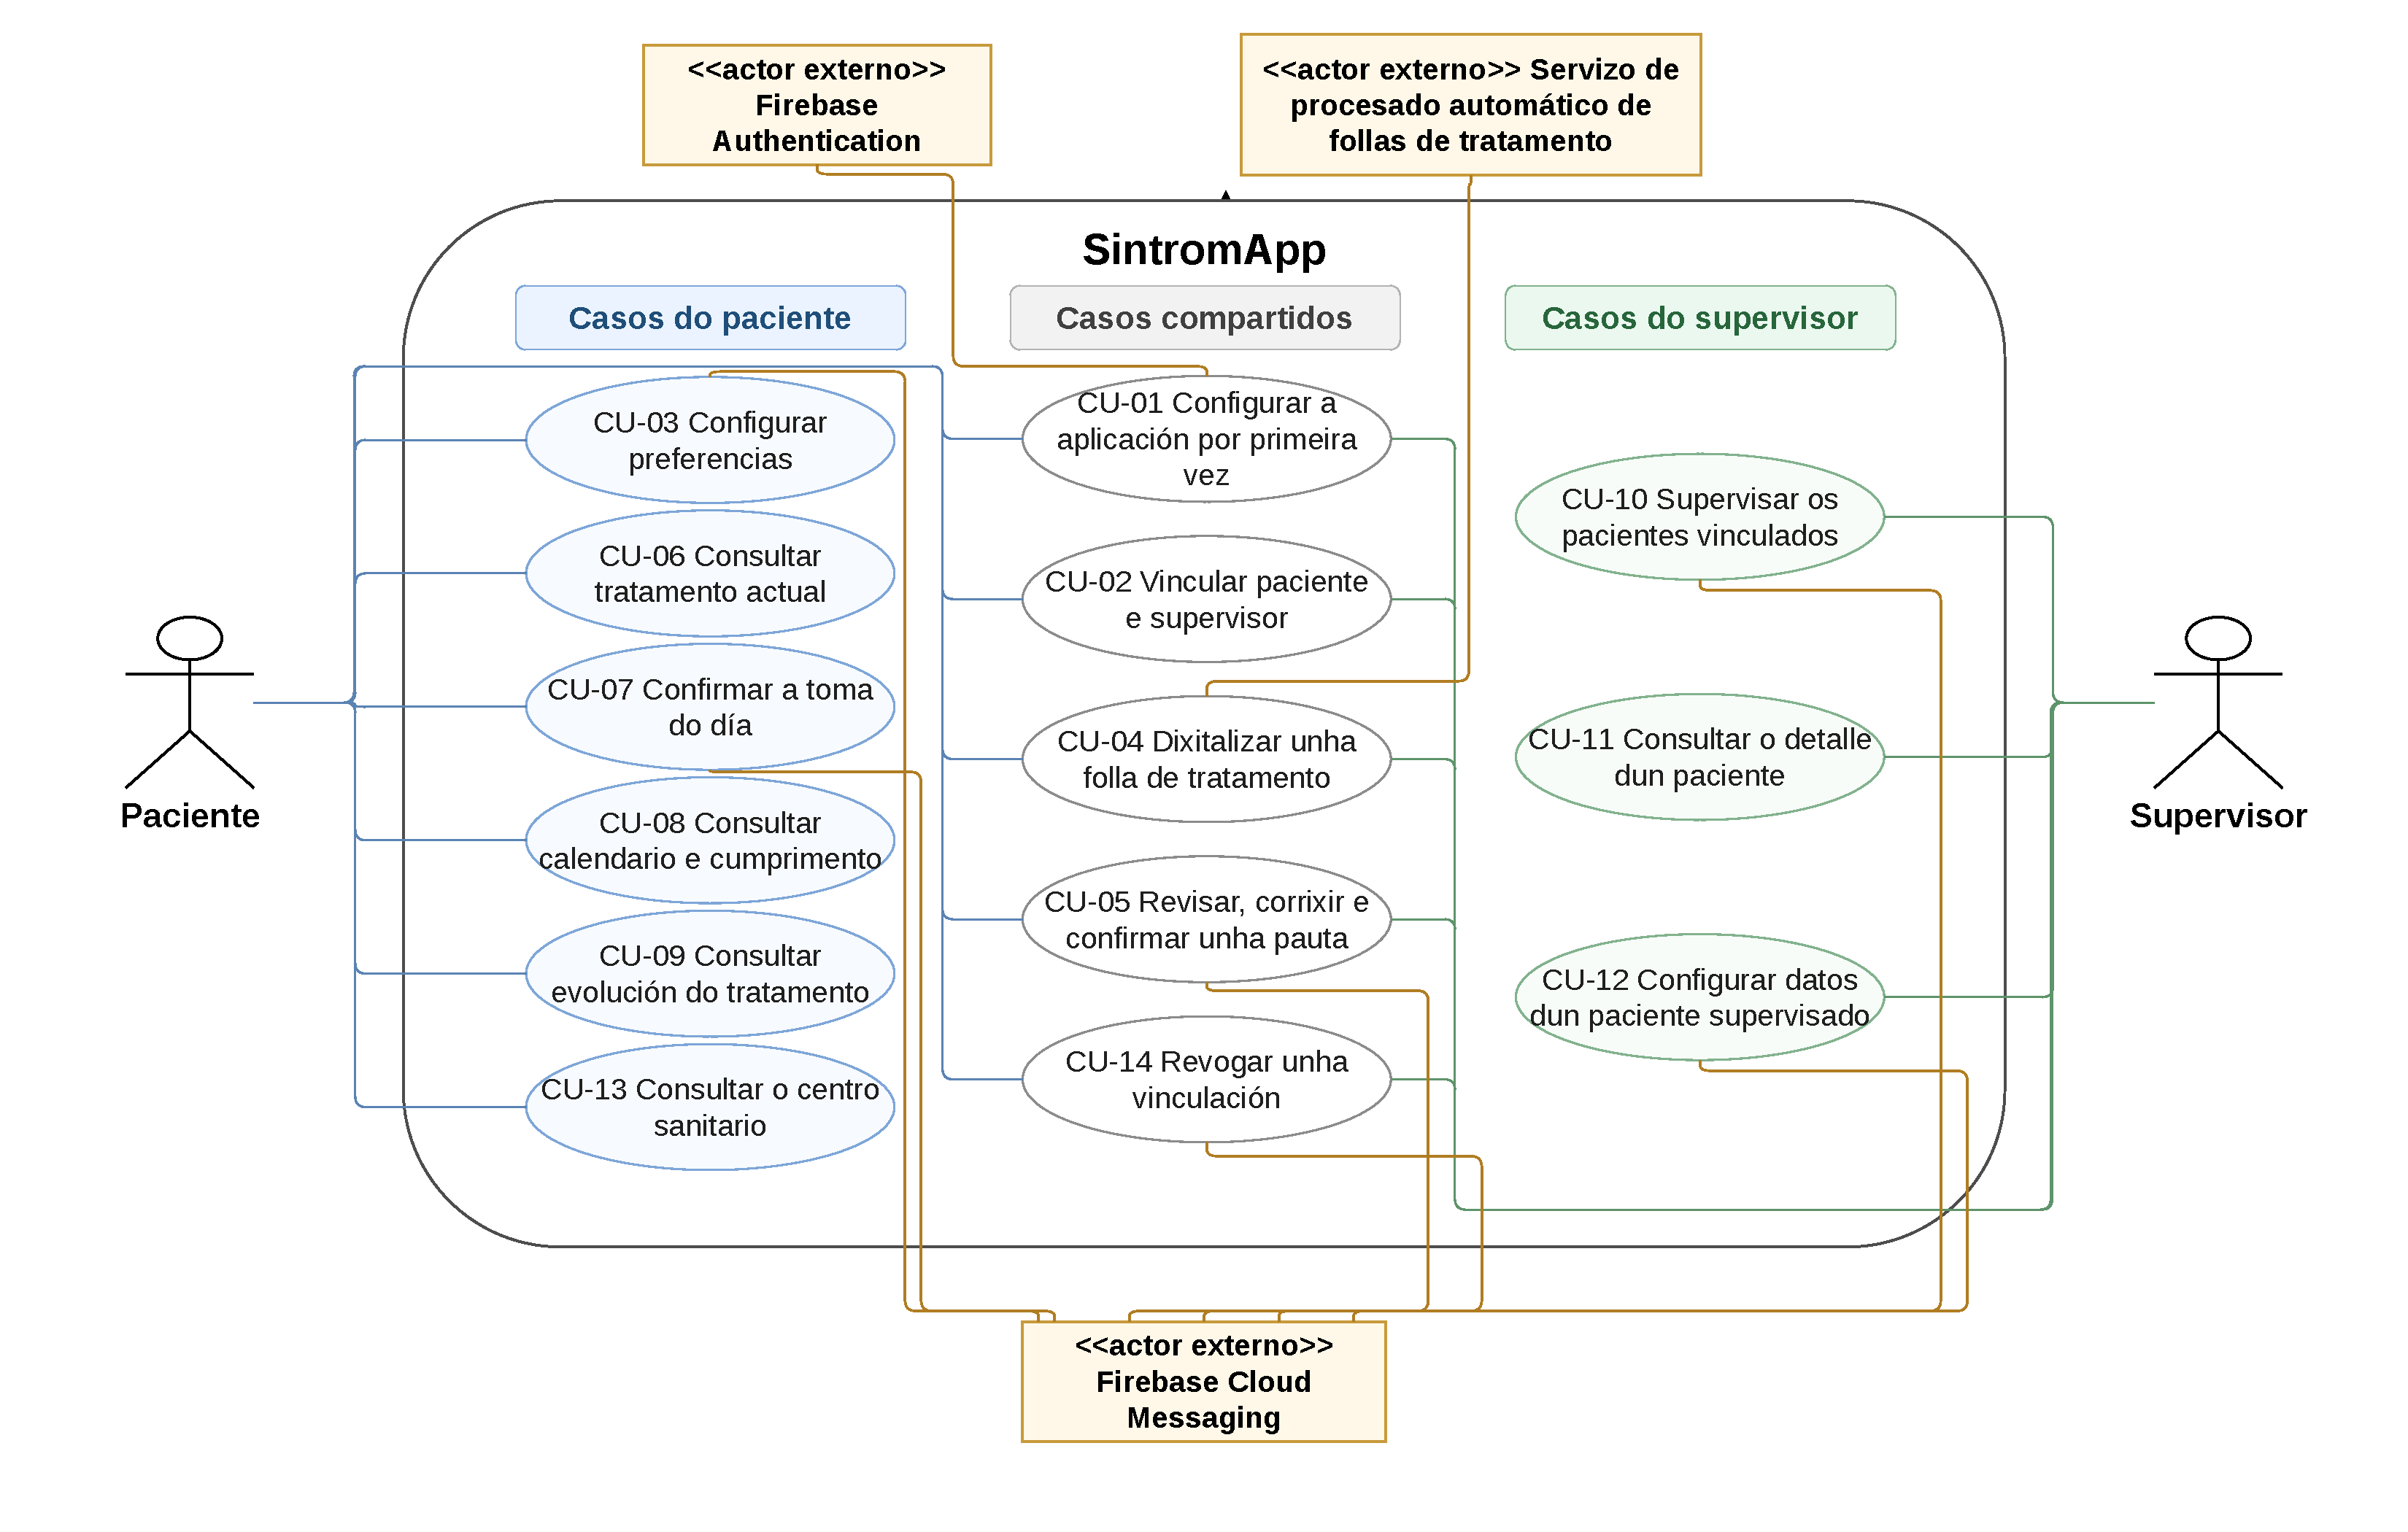
\includegraphics[width=1\linewidth]{imaxes/04-Analise/diagrama_casos_uso_sintromapp_definitivo_letra_moi_grande.drawio.pdf}
\caption{Diagrama dos casos de uso da aplicación}
\label{fig:diagrama-casos-uso}
\end{figure}
